% !TEX root = ../cube_einfty.tex

\section{Operads, props and \texorpdfstring{${E_\infty}$}{E-infty}-structures} \label{s:props}

We now review the definition of the finitely presented prop $\M$ introduced in \cite{medina2020prop1} and whose associated operad is a model of the $E_\infty$-operad.
Given its small number of generators and relations, is well suited to define $E_\infty$-structures.
In the next section we use this model to define natural $E_\infty$-structures on cubical chains and cochains.
We start by reviewing the basic material in the theory of operads and props, referring the reader to, for example, \cite{markl2008props} for a more complete treatment.

\subsection{Symmetric (bi)modules}

Let $\Sym$ be the category whose objects are the non-negative integers $\N$ and whose set of morphisms between $n$ and $n'$ is empty if $n \neq n'$ and is otherwise the symmetric group $\Sym_n$.
A \textit{left $\Sym$-module} (resp. \textit{right} $\Sym$-\textit{module} or $\Sym$-\textit{bimodule}) is a functor from $\Sym$ (resp. $\Sym^\op$ or $\Sym^\op \times \Sym$) to $\Ch$.
In this paper we prioritize left module structures over their right counterparts.
As usual, taking inverses makes both perspectives equivalent.
We respectively denote by $\Symmod$ and $\Symbimod$ the categories of left $\Sym$-modules and of $\Sym$-bimodules with morphisms given by natural transformations.

Given a chain complex $C$, we have the following key examples of a left and a right $\Sym$-module
\begin{gather*}
	\End^C(n) = \Hom(C, C^{\ot n}), \qquad
	\End_C(m) = \Hom(C^{\ot m}, C),
\end{gather*}
and of an $\Sym$-bimodule
\[
\End^C_C(m,n) = \Hom(C^{\ot m}, C^{\ot n}),
\]
where the symmetric actions are given by permutation of tensor factors.

The group homomorphisms $\Sym_n \to \Sym_1^\op \times \Sym_n$ induce a forgetful functor
\begin{equation} \label{e:forgetful}
	\forget \colon \Symbimod \to \Symmod
\end{equation}
defined explicitly on an object $\cP$ by $\forget(\cP)(n) = \cP(1, n)$ for $n \in \N$.
The similarly defined forgetful functor to right $\Sym$-modules will not be considered.

\subsection{Composition structures}

\textit{Operads} and \textit{props} are obtained by enriching $\Sym$-modules and $\Sym$-bimodules with certain composition structures.
Intuitively, these are obtained by abstracting the composition structure naturally present in the left $\Sym$-module $\End^C$ (or right $\Sym$-module $\End_C$), naturally an operad, and the $\Sym$-bimodule $\End^C_C$, naturally a prop.
More explicitly, an operad $\cO$ is a left $\Sym$-module with chain maps
\begin{gather*}
	\k \to \cO(1), \\
	\cO(n_1) \ot \dotsb \ot \cO(n_r) \ot \cO(r) \to \cO(n_1 + \dots + n_r),
\end{gather*}
satisfying relations of associativity, equivariance and unitality.
Similarly, a prop $\cP$ is a $\Sym$-bimodule together with chain maps
\begin{gather*}
	\k \to \cP(n,n), \\
	\cP(m,k) \ot \cP(k,n) \to \cP(m,n), \\
	\cP(m,n) \ot \cP(m',n') \to \cP(m+m',n+n'),
\end{gather*}
satisfying certain natural relations.
For a complete presentation of these concepts we refer to Definition~11 and 54 of \cite{markl2008props}.
We respectively denote the category of operads and props with structure preserving morphisms by $\operads$ and $\props$.

Let $C$ be a chain complex, $\cO$ an operad, and $\cP$ a prop.
An $\cO$-\textit{coalgebra} (resp. $\cO$-\textit{algebra} or $\cP$-\textit{bialgebra}) structure on $C$ is an structure preserving morphism $\cO \to \End^C$ (resp. $\cO \to \End_C$ or $\cP \to \End_C^C$).

We remark that the forgetful functor \eqref{e:forgetful} restricts to
\[
\forget \colon \props \to \operads,
\]
so any $\cP$-bialgebra structure on $C$
\[
\cP \to \biEnd_C^C
\]
induces a $\forget(\cP)$-coalgebra structure on it
\[
\forget(\cP) \to \forget(\biEnd_C^C) \cong \coEnd^C.
\]

\subsection{\texorpdfstring{${E_\infty}$}{E-infty}-operads}

Recall that a \textit{projective $\Sym_n$-resolution} of a chain complex $C$ is a quasi-isomorphism $R \to C$ from a chain complex $R$ of projective $\k[\Sym_n]$-modules.

An $\Sym$-module $M$ is said to be $E_\infty$ if there exists a morphism of $\Sym$-modules $M \to \underline{\k}$ inducing for each $n \in \N$ a free $\Sym_n$-resolution $M(n) \to \k$.
For example, we can obtain one such $\Sym$-module by using the functor of singular chains and the set $\{\mathrm{E} \Sym_n \to \ast\}_{n \in \N}$ of maps to the terminal space from models of the universal $\Sym_n$-bundle.

An operad is said to be an \textit{$E_\infty$-operad} if its underlying $\Sym$-module is $E_\infty$.
A prop $\cP$ is said to be an \textit{$E_\infty$-prop} if $\forget(\cP)$ is an $E_\infty$-operad.

\subsection{Presentations} \label{ss:presentation}

\begin{figure}
	\boxed{\begin{tikzpicture}[scale=.6]
\draw (1,3.7) to (1,3); 

\draw (1,3) to [out=205, in=90] (0,0);

\draw [shorten >= 0cm] (.6,2.73) to [out=-100, in=90] (2,0);

\draw [shorten >= .15cm] (1,3) to [out=-25, in=30, distance=1.1cm] (1,1.5);
\draw [shorten <= .1cm] (1,1.5) to [out=210, in=20] (0,1);

\node at (1,3.9){};
\node at (0,-.32){};
\node at (2,-.32){};

\node at (3,1.5){$\sim$\ \ \ };
\end{tikzpicture}
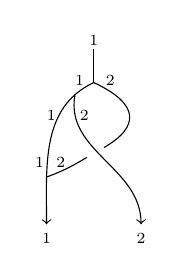
\begin{tikzpicture}[scale=.6]
\draw (1,3.7) to (1,3); 

\draw [->](1,3) to [out=205, in=90] (0,0);

\draw [shorten >= 0cm,->] (.6,2.73) to [out=-100, in=90] (2,0);

\draw [shorten >= .15cm] (1,3) to [out=-25, in=30, distance=1.1cm] (1,1.5);
\draw [shorten <= .1cm] (1,1.5) to [out=210, in=20] (0,1);


\def\x{.8}

\node[scale=\x] at (1,3.9){$\scriptstyle 1$};

\node[scale=\x] at (.7,3.05){$\scriptstyle 1$};
\node[scale=\x] at (1.35,3.05){$\scriptstyle 2$};

\node[scale=\x] at (.1,2.3){$\scriptstyle 1$};
\node[scale=\x] at (.8,2.3){$\scriptstyle 2$};

\node[scale=\x] at (-.15,1.3){$\scriptstyle 1$};
\node[scale=\x] at (.3,1.3){$\scriptstyle 2$};

\node[scale=\x] at (0,-.3){$\scriptstyle 1$};
\node[scale=\x] at (2,-.3){$\scriptstyle 2$};
\end{tikzpicture}}
	\caption{Immersed graphs represent labeled directed graphs with the direction implicitly given from top to bottom and the labeling from left to right.}
	\label{f:immersion}
\end{figure}

The \textit{free prop} $\free(M)$ generated by an $\Sym$-bimodule $M$ is constructed using isomorphism classes of directed graphs with no directed loops that are enriched with the following labeling structure.
We think of each directed edge as built from two compatibly directed half-edges.
For each vertex $v$ of a directed graph $\Gamma$, we have the sets $in(v)$ and $out(v)$ of half-edges that are respectively incoming to and outgoing from $v$.
Half-edges that do not belong to $in(v)$ or $out(v)$ for any $v$ are divided into the disjoint sets $in(\Gamma)$ and $out(\Gamma)$ of incoming and outgoing external half-edges.
For any positive integer $n$ let $\overline{n} = \{1, \dots, n\}$ and set $\overline{0} = \emptyset$.
For any finite set $S$, denote the cardinality of $S$ by $|S|$.
The labeling is given by bijections
\[
\overline{|in(\Gamma)|} \to in(\Gamma), \qquad
\overline{|out(\Gamma)|} \to out(\Gamma),
\]
and
\[
\overline{|in(v)|} \to in(v), \qquad
\overline{|out(v)|} \to out(v),
\]
for every vertex $v$.
We refer to the isomorphism classes of such labeled directed graphs with no directed loops as $(m,n)$\textit{-graphs} denoting the set of these by $\graphs(m,n)$, where $m$ and $n$ denote respectively the number of incoming and outgoing half-edges of any $\Gamma \in \graphs(m,n)$.
We use graphs immersed in the plane to represent elements in $\graphs(m,n)$, please see \cref{f:immersion}.
We consider the right action of $\Sym_m$ and the left action of $\Sym_n$ on a $(m,n)$-graph given respectively by permuting the labels of $in(\Gamma)$ and $out(\Gamma)$.
This action defines the $\Sym$-bimodule structure on the free prop
\begin{equation} \label{e:free prop}
\free(M)(m,n) \ =
\bigoplus_{\Gamma \in \graphs(m,n)} \
\bigotimes_{v \in Vert(\Gamma)} out(v) \ot_{\Sym_p} M(p, q) \ot_{\Sym_p} in(v),
\end{equation}
where we simplified the notation writing $p$ and $q$ for $\overline{|in(v)|}$ and $\overline{|out(v)|}$ respectively, the differential $\bd_{\free(M)}$ is the extension of that of $M$ to the tensor product \eqref{e:free prop}, and the composition structure is defined by
\[
\begin{tikzcd}[column sep=small, row sep=0]
	\k \arrow[r]& \free(M)(r,r) \\
	1 \arrow[r, mapsto] & \identity \ \identity \dotsb \identity
\end{tikzcd}
\]
and (relabeled) grafting and disjoint union.

Let $G$ be assignment of a set $G(m,n)_d$ to each $m,n \in \N$ and $d \in \Z$.
Denote by $\k[\Sym^\op \times \Sym] \set{G}$ the $\Sym$-bimodule assigning to $(m,n)$
the chain complex with trivial differential and degree $d$ part equal to
\[
\k[\Sym^\op_m \times \Sym_n] \set[\big]{G(m,n)_d}.
\]
We will denote by $\free(G)$ the free prop generated by this $\Sym$-bimodule.
Let $\bd \colon \k[\Sym^\op \times \Sym] \set{G} \to \free(G)$ be a morphism of $\Sym$-bimodule whose monoidal extension $\bd \colon \free(G) \to \free(G)$ defines a differential.
We denote by $\free_{\bd}(G)$ the prop obtained by endowing $\free(G)$ with this differential.
Let $R$ be a collection of elements in $\free(G)$ and denote by $\angles{R}$ the smallest ideal containing $R$.
The prop \textit{generated by $G$ modulo $R$ with boundary $\bd$} is defined to be $\free_{\bd}(G) \big/ \angles{R}$.

\subsection{The prop $\M$}

We now recall the $E_\infty$-prop that is central to our constructions.

\begin{definition}
	Let $\M$ be the prop generated by
	\begin{equation} \label{e:generators of M}
	\counit \,, \qquad
	\coproduct \,, \qquad
	\product,
	\end{equation}
	in $(1,0)_0$\,, $(1,2)_0$ and $(2,1)_1$ respectively,
	modulo the relations
	\begin{equation} \label{e:relations of M}
		\leftcounitality \,, \qquad
		\rightcounitality \,, \qquad
		\productcounit,
	\end{equation}
	with boundary defined by
	\begin{equation} \label{e:boundary of M}
	\bd\ \counit = 0, \qquad
	\bd\, \coproduct = 0, \qquad
	\bd \product = \ \boundary\,.
	\end{equation}
\end{definition}

Explicitly, any element in $\M(m,n)$ can be written as a linear combination of the $(m,n)$-graphs generated by those in \eqref{e:generators of M} via grafting, disjoint union and relabeling, modulo the prop ideal generated by the relations in \eqref{e:relations of M}. Its boundary is determined by \eqref{e:boundary of M} using \eqref{e:free prop}.

\begin{proposition}[{\cite[Theorem 3.3]{medina2020prop1}}]
	$\M$ is an $E_\infty$-prop.
\end{proposition}

\begin{remark*}
	The prop $\Med$ is obtained from applying the functor of chains to a prop over the category of cellular spaces \cite{medina2021prop2} which can be thought of as a resolution of the operad of stable arc surfaces \cite{kaufmann2009dimension}.
\end{remark*}
